% Chapter Template

\chapter{Design and Implementation} % Main chapter title

\label{Chapter5} % Change X to a consecutive number; for referencing this chapter elsewhere, use \ref{ChapterX}

\lhead{Chapter 5. \emph{Design \& Implementation}} % Change X to a consecutive number; this is for the header on each page - perhaps a shortened title


In this chapter we will go over the implementation process of the project. We will describe various choices we made, justifying them in the context of our objectives. 

First we will describe our solution to the mood detection problem. We first try to determine which musical features are the most correlated to the AV values of the music's emotion. Then, by training a neural network with data containing chosen features we will create a way of determining the arousal and valence value of any musical track, which will be later used in the implementation of our game. In addition to this, by investigating the impact of different parameters we will make sure out network has as good performance and accuracy as possible.

Next, we will move on to main melody detection by looking at two algorithms - one using source separation based approach and the other using the salience based approach. We will evaluate performance of both of them on data from recent pop culture to determine their performance and fitness in this project.

The next section will describe our attempt to automated music segmentation.

Last, but not least, we will talk about the game itself, its architecture, flow of use and design choices made.

\vspace{20pt}

\section{Mood Detection}

A common reason for engaging in music listening is that music is an effective means of conveying and evoking emotions. Although they may be subjective, based in part on the listener’s cultural and musical background or preferences, there are commonalities in perceived emotion across different listeners based on the characteristics of the music. Several studies have attempted to predict emotion conveyed during music listening. In our approach, we decided to represent the emotion connected to the music using a two-dimensional space with valence on the x-axis and arousal on the y-axis, first proposed by R. E. Thayer \cite{Thayer}.

As we described in Section \ref{sec:emotionClass}, there is a relation between valence and arousal values for a musical track and the moods perceived by people. In essence, the high arousal is connected to how energetic the music is, whereas valence refers to how positive (or negative) the emotions in the track are. 

\vspace{10pt}

\subsection{Choice of Features}
Using Essentia library \cite{essentia}, we implemented an extractor to retrieve certain features from a song, which we would expect to have certain impact on the perceived mood of a musical piece:

\begin{description}

\item[average loudness] - dynamic range descriptor. It rescales average loudness into the [0,1] interval on a per window basis. The value of 0 corresponds to signals with large dynamic range, 1 corresponds to signal with little dynamic range. This could indicate the level of the arousal, with higher loudness implying higher arousal value. We believe this relation could be quite intuitive - sad or peaceful songs tend to be quiet whereas excited or angry emotions are usually linked to louder tracks.

\item[means and derivatives of variance of rates of silent frames] in a signal for thresholds of 20, 30 and 60db. We believe that the values could influence the arousal levels, as the more and the bigger the silent gaps, the sadder / more peaceful the track seems to be, implying the low arousal value. When examining multiple musical tracks we have noticed that the happier or angrier songs can also have such silent gaps, but they tend to be much shorter.

\item[dynamic complexity] - computed on 2 second windows with 1 second overlap. The dynamic complexity is the average absolute deviation from the global loudness level estimate on the dB scale. It is related to the dynamic range and to the amount of fluctuation in loudness present in a recording. We believe this feature would have an impact on both examined values. However, similarly to the loudness level, arousal should be influenced more - as more dynamic songs (excited or angry) are more likely to suffer from loudness changes, whereas more phlegmatic ones (sad or peaceful) tend to keep the same dynamic complexity level.

\item[BPM] - beats per minute value according to detected beats. This feature should be correlated with the arousal level - intuitively, the faster the song, the more energetic it seems. 

\item[spectral centroid] - centroid statistics describing the spectral shape. It indicates where the ``center of mass'' of the spectrum is. Perceptually, it has a robust connection with the impression of ``brightness'' of a sound - an indication of the amount of high-frequency content in a sound. Timbre researchers consider brightness to be one of the perceptually strongest distinctions between sounds \cite{timber}, and formalize it acoustically as an indication of the amount of high-frequency content in a sound. That is why we believe the spectral centroid might be related to both valence and arousal.

\item[spectral RMS] (root mean square) - in physics it is a value characteristic of a continuously varying quantity, such as a cyclically alternating electric current or a sound. It is obtained by taking the mean of the squares of the instantaneous values during its duration or a cycle. This is linked to the loudness of the sound. This is why we believe that it might have an impact on arousal, but we do not exclude its impact on valence.

\item[spectral energy] - the energy E{s} of a continuous-time signal x(t) defined as: 
\begin{equation}
E{s}  =  \langle x(t), x(t)\rangle =  \int_{-\infty}^{\infty}{|x(t)|^2}dt
\end{equation}

Signal energy is always equal to the summation across all frequency components of the signal's spectral energy density. 
There have been some research focusing on relation between spectral energy and singing voice. In particular, in their paper \cite{spectralenergy}, S. Ferguson, D. T. Kenny and D. Cabrera were investigating the relation between the value and the experience of male singers. This makes for an interesting case worth considering in our research.

\item[mean and derivative of variance of beat loudness] -  spectral energy computed on beats segments of audio across the whole spectrum, and ratios of energy in 6 frequency bands. We suspect that the low value of the beat loudness could imply a low arousal.

\item[key and its scale] estimated key and its scale (major or minor) using Temperley’s profile. 
In music theory, the term key is used in many different and sometimes contradictory ways. A common use is to speak of music as being 'in' a specific key, such as ``in the key of C major or in the key of F\#''. Sometimes the terms 'major' or 'minor' are appended, as 'in the key of A minor' or 'in the key of B major'.
Broadly speaking the phrase 'in key of C' means that C is music's harmonic center or tonic (the first degree of the scale, or the root of the scale). 
The terms 'major' and 'minor' further imply the use of a major scale or a minor scale. Thus the phrase 'in the key of E major' implies a piece of tonal music harmonically centered on the note E and making use of a major scale whose first note, or tonic, is E. 
We believe that those features can have an impact on both arousal and valence - songs performed in minor scale are traditionally connected to being sad, whereas the major scale is usually linked to positive emotions.

\item[scale and key of the chords] taken as the most frequent chord, and scale of the progression, whether major or minor. Scale commonly known to have a big influence on our perception on music \cite{keys}. It seems to be mostly the result of cultural conditioning as when people listen to tunes, they rely heavily on their memory. Such constant stimulus to our musical memory helps to generate expectations of what might come next in a tune or preserve the sound - emotion relation.

\item[means of zero-crossing rate] - the rate of sign-changes along a signal, i.e., the rate at which the signal changes from positive to negative or back. This feature has been used heavily in music information retrieval, being a key feature to classify percussive sounds. We believe it could be related to the arousal value. Music has a fairly normal distribution of frames with lower and higher zero-crossing rates. Speech however displays a much more skewed distribution. This could have an impact on songs where the vocals are quite rapid and energetic, for example rap music, and therefore might have a significant impact on mood recognition in our system.
ZCR is defined formally as: 
\begin{equation}
ZCR = \frac{1}{T-1} \sum_{t=1}^{T-1} {{\mathbb I}\left\{{s_t s_{t-1} < 0}\right\}}
\end{equation}

\item[pitch salience of a spectrum] - given by the ratio of the highest auto correlation value of the spectrum to the non-shifted auto correlation value.  Unpitched sounds (non-musical sound effects) and pure tones have an average pitch salience value close to 0 whereas sounds containing several harmonics in the spectrum tend to have a higher value. We think the value could have an effect on both the valence and arousal as pitch salience is often described as the probability of noticing a tone or clarity or strength of tone sensation.

\item[mean and derivative of variance of sensory dissonance] (to distinguish from musical or theoretical dissonance) of an audio signal given its spectral peaks. Sensory dissonance measures perceptual roughness of the sound and is based on the roughness of its spectral peaks. Given the spectral peaks, the algorithm estimates total dissonance by summing up the normalized dissonance values for each pair of peaks. These values are computed using dissonance curves, which define dissonance between two spectral peaks according to their frequency and amplitude relations. Dissonance could be related to low valence.

\end{description}

\begin{figure}
        \centering
        \begin{subfigure}[b]{0.48\textwidth}
                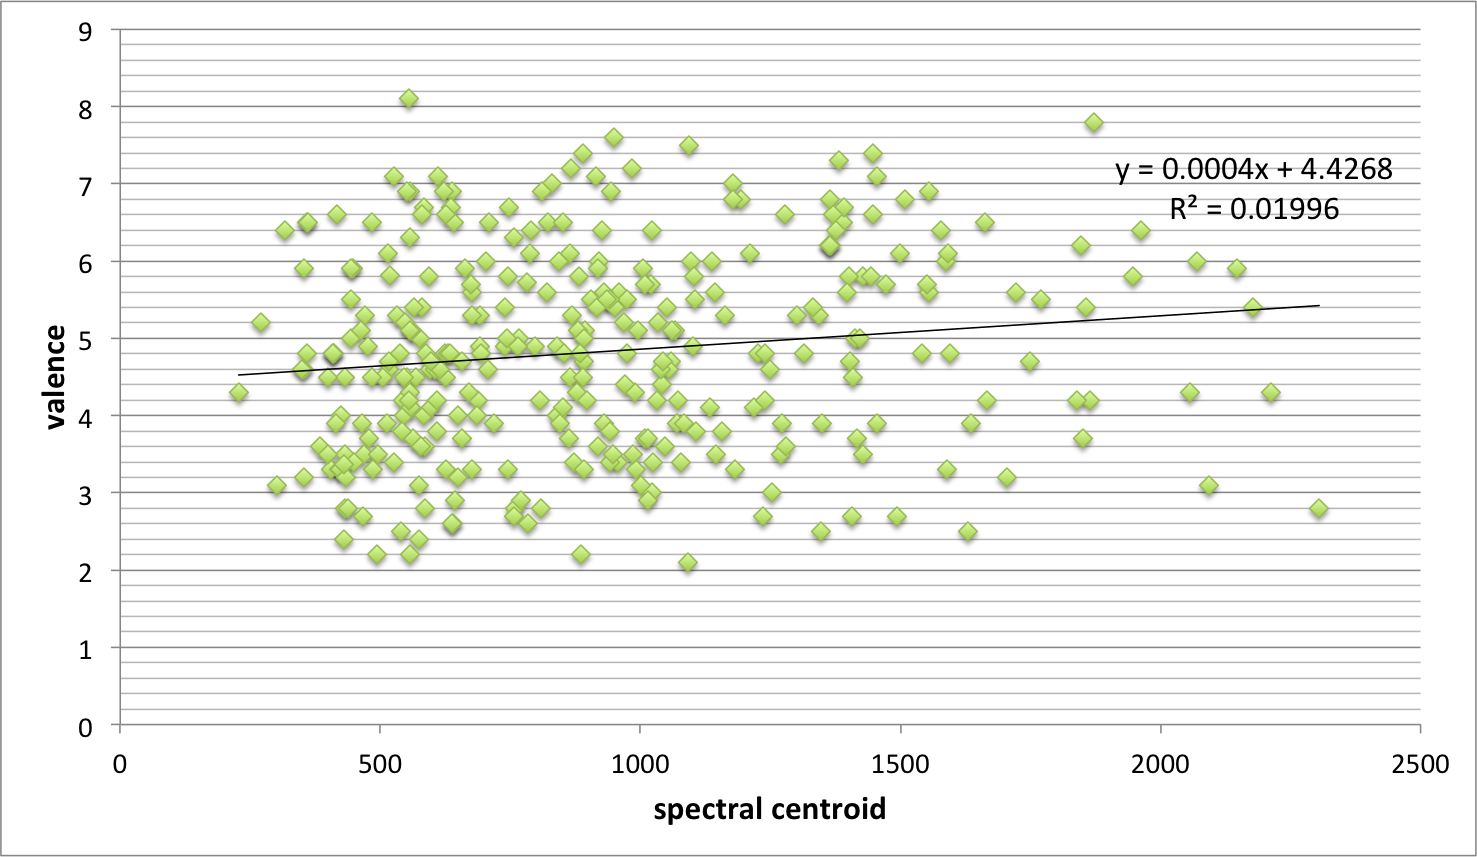
\includegraphics[width=\textwidth]{Figures/spectralcentroid-valence}
                \caption{A graph representing a correlation between spectral centroid and valence values.}
                \label{fig:is }
        \end{subfigure}%
        ~ %add desired spacing between images, e. g. ~, \quad, \qquad, \hfill etc.
          %(or a blank line to force the subfigure onto a new line)
        \begin{subfigure}[b]{0.48\textwidth}
                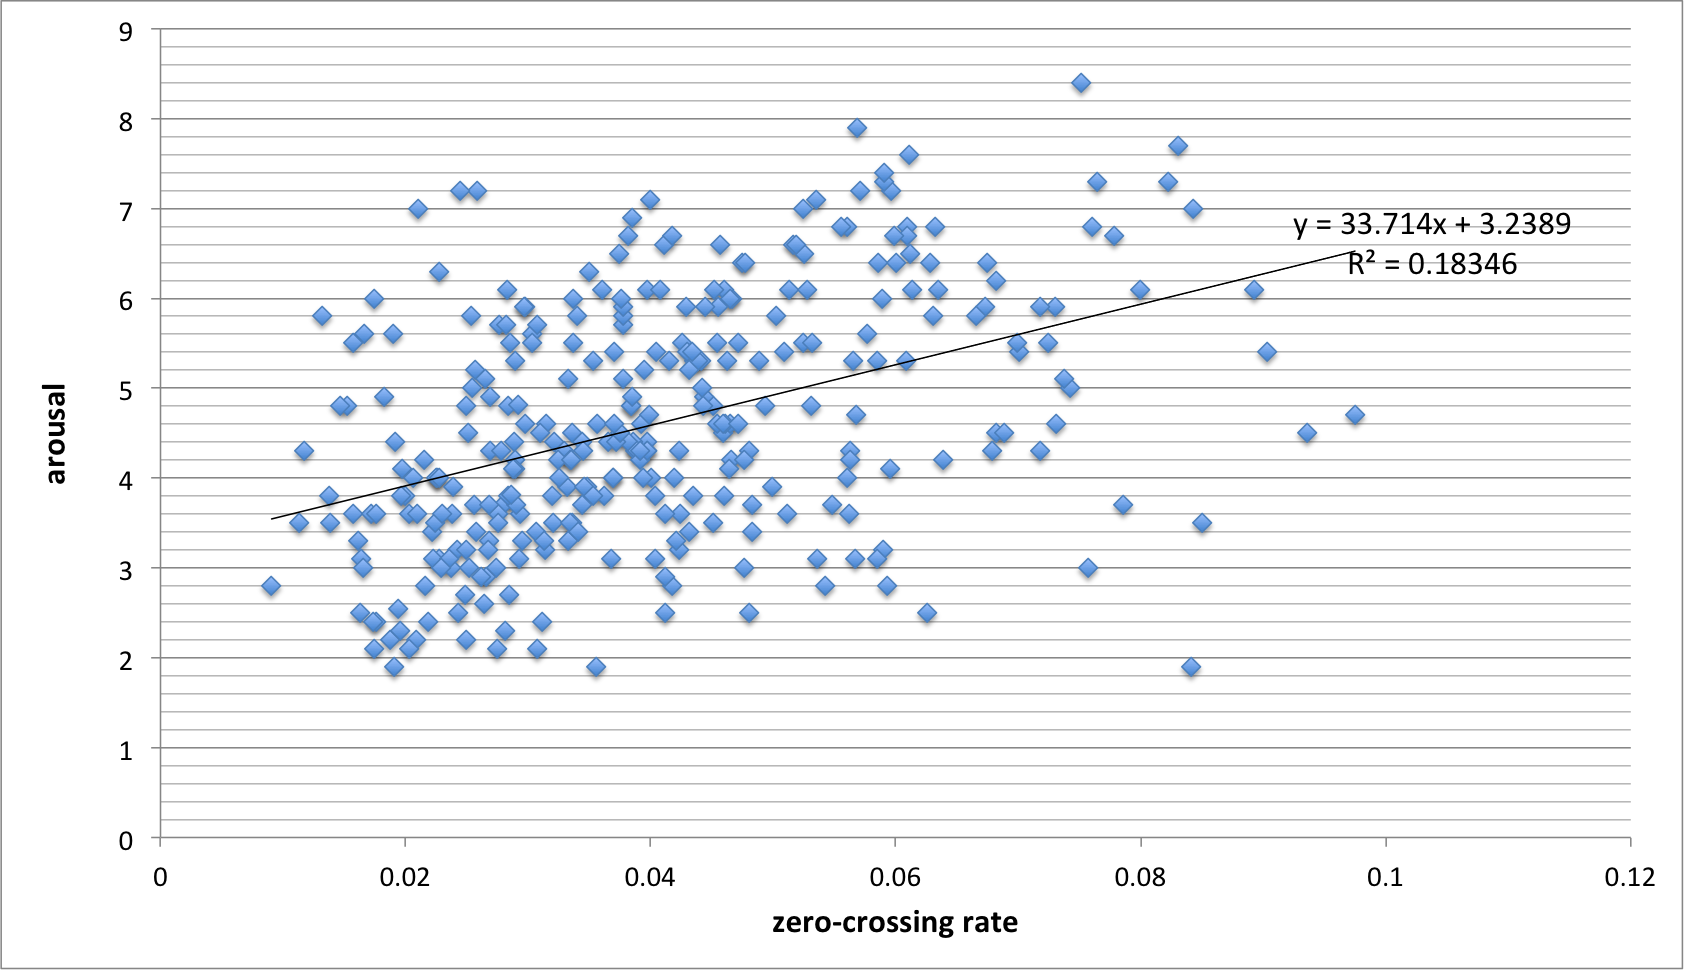
\includegraphics[width=\textwidth]{Figures/zerocrossing-arousal}
                \caption{A graph representing a correlation between zero-crossing rate and arousal values.}
        \end{subfigure}
          \caption{Chosen results of bivariate correlation with multiple regression.}
        ~ %add desired spacing between images, e. g. ~, \quad, \qquad, \hfill etc.
                        \label{fig:bivariateNN}

\end{figure}

\vspace{10pt}

\subsection{Correlation Between Features and Mood Perception}

In our exploration we decided to base our research on data collected in ``1000 Songs for Emotional Analysis of Music'' music library \cite{1000songs}, to avoid personal bias in assessing the mood of the song. The songs in the dataset were annotated by more than 300 crowdworkers on Amazon Mechanical Turk. Each song was annotated for arousal and for valence separately.

As a first step towards understanding the pattern by which audio features might account for emotion ratings, we conducted correlational analyses between features and mean valence/arousal ratings from the data set. We performed a bivariate correlation analysis with the valence/arousal ratings as the dependent variable, and each of the 22 features as the explanatory variable. Example of the results we achieved can be seen in Figure \ref{fig:bivariateNN}, the rest are included in Appendix A (Chapter \ref{sec:appendixa}, Section \ref{sec:bivariatediagram}) for reference. 

We found significant correlation between \textbf{valence} and derivative of varriance and mean \textit{silence60}, derivative of variance of \textit{silence30, dynamic complexity, spectral centroid, spectral RMS, spectral energy, zero-crossing rate, pitch salience, and both mean and dvar of dissonance}. 

For \textbf{arousal}, we noticed correlation with \textit{spectral centroid, pitch salience, zero-crossing rate}, both \textit{mean} and \textit{dva}r of  \textit{silence60, spectral energy, mean dissonance} and \textit{dynamic complexity}. 

Values of all the features were then normalized between 0 and 1 to prepare them for the neural network training. 



\begin{wrapfigure}{l}{0.5\textwidth}
  \vspace{-30pt}
  \begin{center}
    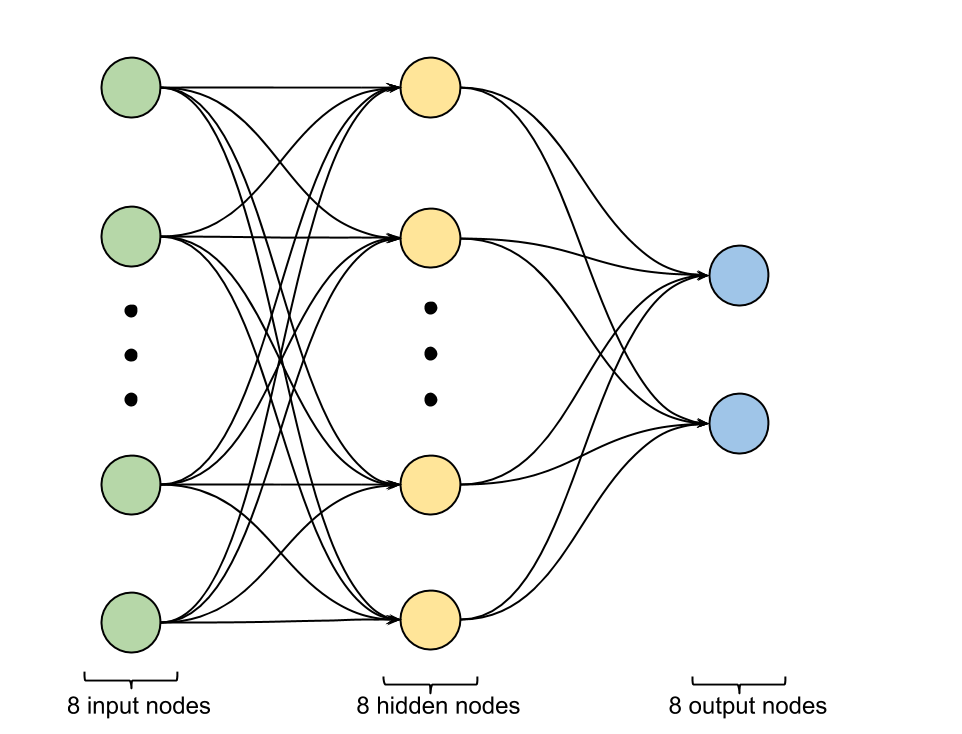
\includegraphics[width=0.5\textwidth]{Figures/myANN}
  \end{center}
  \caption{A diagram depicting the structure of our artificial neural network for mood detection.}
\label{finalnetwork}
\end{wrapfigure}

\vspace{10pt}

\subsection{Neural Network for Mood Prediction}

Our goal was to train the network to predict mean participant valence and arousal values for musical excerpts. 
Our first network implementation was a supervised, feedforward network with backpropagation. 
The input consisted of normalized values of 8 features:
\textit{spectral centroid, pitch salience, zero-crossing rate, silence60 mean  and dvar, mean dissonance, dynamic complexity} and \textit{spectral energy}. 
The network had two outputs - arousal and valence.

As all the training data was normalised, the input and output values were within a range of 0 to 1. The training set consisted of 50 input and output arrays. Each input array had 8 values, one per audio feature, and its corresponding output array had the two desired arousal and valence values.

The network’s task was to provide the valence and arousal values based on the 13 audio features. The output values fell within a range of 0 to 1. Since desired outputs were average valence/arousal ratings provided by participants on a scale from 1 to 9, the network outputs were rescaled back. The training set consisted of eight input and output arrays. Each input array had 13 values, one for each audio feature, and its corresponding output array had the two desired arousal and valence values. The connection weights from input to the hidden nodes and from hidden nodes to the output ones were initialised to random numbers. 

The network was built, trained, and tested using the pyBrain python library for neural network implementation. 

We trained our network for 1000 epochs with many different sizes of the hidden layer and default values for all the other parameters. The performance based on that can be seen in Table \ref{table:rsmetable}.

\begin{figure}[h]
	\centering
   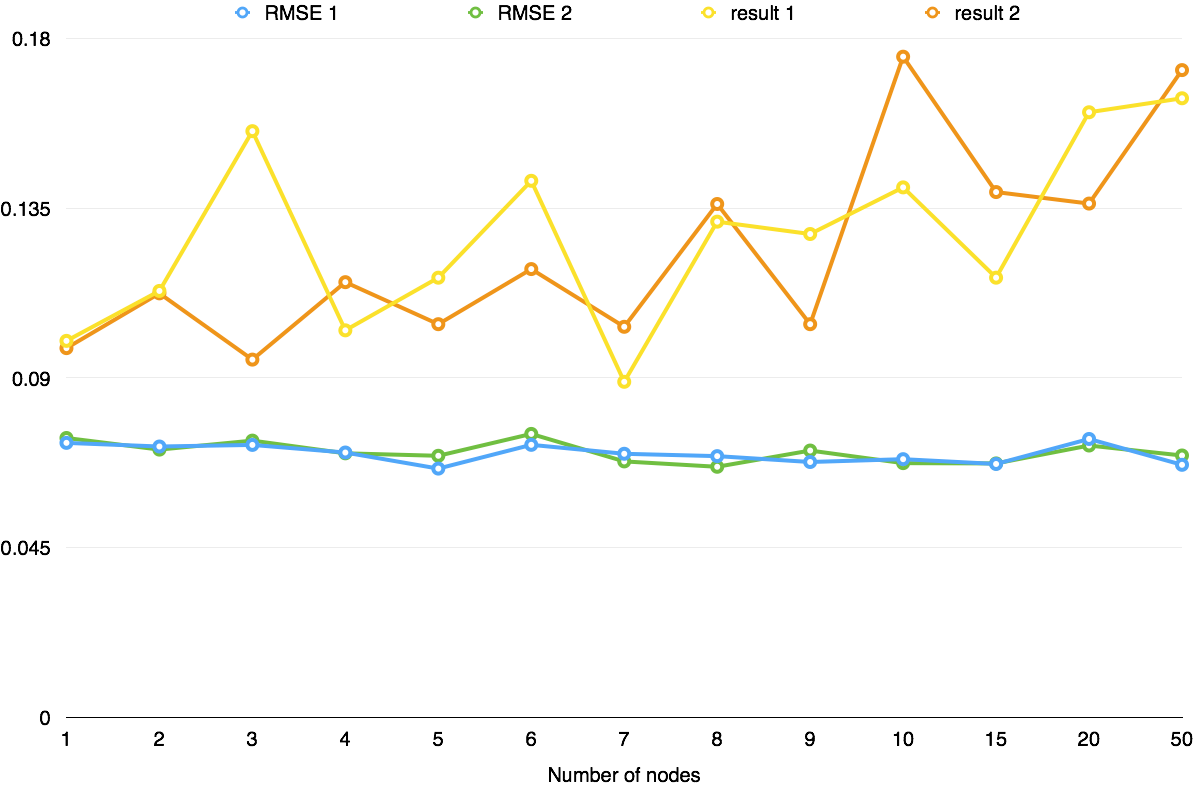
\includegraphics[width=0.7\textwidth]{Figures/nodesperf}
\caption{Data presented in table \ref{table:rsmetable}, plotted on a diagram.}
\end{figure}


\begin{table}
\begin{center}
\begin{tabular}{| c | l | l | l | l |} \hline 
  No. of Nodes & RMSE 1 & RMSE 2 & result 1 & result 2  \\ \hline \hline
  1 &  0.0727638005274 & 0.0740582536152  & 0.0998088934575 & 0.0978822145006 \\ \hline
  2 &  0.071796654024 & 0.0709793303052 & 0.113046836083 & 0.112405435125 \\ \hline
  3 & 0.0722212571658 & 0.0733605257262 &  0.155412522783 & 0.0948392717258 \\ \hline
  4 &   0.0702013899702 & 0.0699921976435 &  0.102602437509 & 0.115373051966 \\ \hline
  5 &  0.0659433293266 &  0.0693361162261 &  0.116558760273  & 0.10423200269\\ \hline
  6 & 	 0.0722427034758 & 0.0751383013205 &  0.142248432275  &  0.118843096333  \\ \hline
  7 &  0.0698701385354  & 0.0678483277007  & 0.088954243616 & 0.103537259056 \\ \hline
  8 &   0.0692459138916 &  0.066424019477 & 0.131412928439 & 0.136098090028 \\ \hline
  9 &   0.0676910853628 &  0.0707274913708 & 0.128139548772 & 0.104231713578\\ \hline
 10 & 0.0684398705278 & 0.0673887116962 & 0.140505458102 & 0.175156506583\\ \hline
 15 & 0.0671656450239 & 0.0673141803371 & 0.116563143115  &  0.139265837027\\ \hline
 20 & 0.0737978227013 &  0.0720620813131 & 0.160424096589 & 0.136210925296\\ \hline
 50 & 0.0669456166054 &   0.0694139442297 & 0.164132829293 & 0.171603556123\\ \hline
\end{tabular}
\caption{Table showing the root mean square error for training the network for given number of nodes in the hidden layer.}
\label{table:rsmetable}
\end{center}
\end{table}


As we can see, the optimal solution is the one with 7 nodes in the hidden layer. Although the initial RMSE returned after training is not overall minimum, all the values - so both the training ones and the ones after the evaluation, are local minimas and one of the minimal values overall. This decision can be justified by the fact that altough for some cases we managed to achieve smaller RSME from the training, the network was in fact overfitting, and doing really well for the already known input, but worse for a new one.
To avoid overfitting the network, we kept the number of hidden units equal to the number of input units. 

\begin{table}
\begin{center}
\begin{tabular} {| c | l | l |} \hline
 Learning Rate & RMSE & result RMSE \\  \hline \hline
 0.3 & 0.0707970888752 & 0.14578838717 \\ \hline
 0.25 & 0.0699336891245 & 0.163193322998 \\ \hline
 0.2 &  0.0667986974361 & 0.15521882498 \\ \hline
 0.15 & 0.0724218948598 & 0.104971086068 \\ \hline
 0.1 & 0.0684257582616 & 0.100719004205 \\ \hline
 0.05 & 0.0695957657331 & 0.0979349713899 \\ \hline
 0.01 & 0.0689460348924 & 0.090954243616 \\ \hline
 0.005 & 0.0724023992534 & 0.130733683966 \\ \hline
 0.001 &  0.079664786995 & 0.112619882406 \\ \hline
\end{tabular}
\caption{Table showing the root mean square error for training the network for given learning rate parameter value.}
\label{table:learningrate}
\end{center}
\end{table}

\begin{figure}[h]
	\centering
   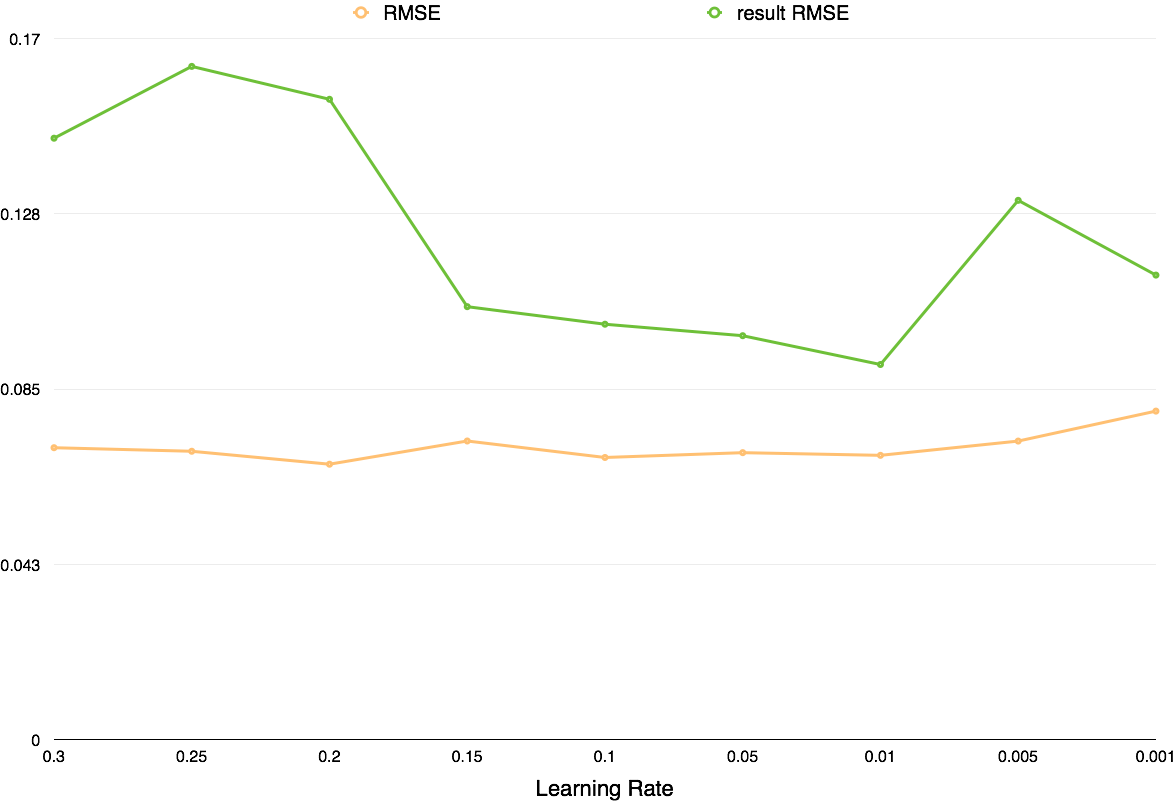
\includegraphics[width=0.7\textwidth]{Figures/learningrate}
\caption{Data presented in table \ref{table:learningrate}, plotted on a diagram.}
\end{figure}


Having found the optimal number of nodes in the hidden layer, we moved on to find the learning rate parameter. We started our search by setting it to 0.3 and reducing it over time. The results we found can be found in Table \ref{table:learningrate}. As we can see, the optimal solution seems to be learning rate at value 0.001.


In the end, we came up with the network which can be seen on Figure \ref{fig:finalnetwork}.

\vspace{20pt}

\section{Main Melody Extraction}

\vspace{10pt}

\section{Structure Retrieval}

Understanding the structure of music (e.g. intro, verse, chorus, bridge, and outro) is important as it allows us to divide a song into semantically meaningful segments, within which musical characteristics are relatively consistent.

\vspace{10pt}

\subsection{Feature Choice}

To implement a system capable of unsupervised structure recognition, we need to provide it with some data. We investigated two possible values - \textit{Mel-frequency cepstral coefficients} and \textit{harmonic pitch class profile}.

Cepstrum is the result of taking the Inverse Fourier transform (IFT) of the logarithm of the estimated spectrum of a signal. It can be viewed as information about rate of change in the different spectrum bands.

The mel-frequency cepstrum (MFC) is a representation of the short-term power spectrum of a sound, based on a linear cosine transform of a log power spectrum on a nonlinear mel scale of frequency.

\textit{Mel-frequency cepstral coefficients} (MFCCs) are coefficients that collectively make up an MFC. They are increasingly finding uses in music information retrieval applications such as genre classification, audio similarity measures, etc.

MFCCs are derived from a type of cepstral representation of the audio clip. The mel-frequency cepstrum differs from cepstrum by having its frequency bands equally spaced on the mel scale, which approximates the human auditory system's response more closely than the linearly-spaced frequency bands used in the normal cepstrum. This frequency warping can allow for better representation of sound, for example, in audio compression.

MFCCs are commonly derived as follows:
\begin{itemize}
\item Take the Fourier transform of a signal.
\item Map the powers of the spectrum obtained above onto the mel scale, using triangular overlapping windows.
\item Take the logs of the powers at each of the mel frequencies.
\item Take the discrete cosine transform of the list of mel log powers, as if it were a signal.
\item The MFCCs are the amplitudes of the resulting spectrum.
\end{itemize}

An alternative to using MFCCs as the features to base the algorithm on is \textit{HPCP}.

Harmonic pitch class profiles (HPCP) is a vector of features extracted from an audio signal, based on the Pitch Class Profile descriptor. HPCP is an enhanced pitch distribution feature which is a sequence of chroma - feature vectors describing tonality measuring the relative intensity of each of the 12 pitch classes of the equal-tempered scale within an analysis frame. 

HPCP features can be found and used to estimate the key of a piece, to measure similarity between two musical pieces and to classify music in terms of composer, genre or mood. The process is related to time-frequency analysis. In general, chroma features are robust to noise, for example an ambient noise or percussive sounds, independent of timbre and instrumentation and independent of loudness and dynamics.

The General HPCP feature extraction procedure is summarized as follows:
\begin{itemize}
\item Input musical signal.
\item Do spectral analysis to obtain the frequency components of the music signal.
\item Use Fourier transform to convert the signal into a spectrogram. (The Fourier transform is a type of time-frequency analysis.)
\item Do frequency filtering. A frequency range of between 100 and 5000 Hz is used.
\item Do peak detection. Only the local maximum values of the spectrum are considered.
\item Do reference frequency computation procedure. Estimate the deviation with respect to 440 Hz.
\item Do Pitch class mapping with respect to the estimated reference frequency. This is a procedure for determining the pitch class value from frequency values. A weighting scheme with cosine function is used. It considers the presence of harmonic frequencies (harmonic summation procedure), taking account a total of 8 harmonics for each frequency. In order to map the value on a one-third of a semitone, the size of the pitch class distribution vectors has to be equal to 36.
\item Normalize the feature frame by frame dividing through the maximum value to eliminate dependency on global loudness.
\end{itemize}

The discussion of results given each of the alternatives are discussed in Section \ref{sec:structurefeatures}.

\vspace{10pt}

\subsection{Feature Preparation}

A series of transformations are applied to the data in order to better distinguish the different parts of a song. First, we need to we synchronise our data with with the beats detected in the musical track. sensitive to local noise signal and chord variations [25]. To reduce local variation one can apply beat synchronization, a process of summarizing (usually taking the mean/median of) frame-wise features that occur between two beats, yielding fewer but longer beat-syn- chronous frames [7], [26]. The rationale for doing this is that chord labels between two consecutive beats tend to be the same; hence, the use of a beat-synchronous frame eliminates the effect of local variation. A recent approach related to this is to consider the boundary information pro- vided by repeated segments of a song, then smoothing chroma vectors corresponding to the same repetition to re- duce variation [20].


Moreover, we resample onset-based asynchronous chroma features (as found through The Echo Nest track API) to beats, thus reducing greatly the number of frames across the musical piece, and leading to beat-synchronous chromagrams.

 First, a sliding median filter of size h is run against each of the beat-synchronous chromagram channels. The median filter gives sharper edges than a regular mean filter, which is useful in obtaining sec- tion boundary precision. By filtering features across time, we retain the most prominent chromas within the h-size window and remove smaller artifacts, which are irrelevant in our con- text. In Figure 1 we show the example of a non-filtered and its corresponding pre-filtered chromagram.

We then compute the SSM of the pre-filtered beat- synchronous chromagram. The SSM gives us pair-wise com- parisons of a given set of features using a specific distance measure and stores the results in an N x N symmetric matrix D, such that D(i, j) holds the distance between the features of the beat indices i and j. In this case D(i,j) = D(j,i) and D(i,i) = 0. It is essentially a specific instance of the more generic recurrence plots [16], but using distances (or similarities) instead of binary values. In our experiments we found that the Correlation distance gave better results than other distances, including the Euclidean, Cosine or Manhat- tan distance. The correlation distance is defined as follows:
where || dot ||2 stands for the Euclidean distance, miu x denotes the mean of the feature vector x, and · represents the dot prod- uct.

Finally, we enhance the SSM by using a power-law ex- pansion (using the power 2 empirically gave us the best results), such that close similarities will be closer and distant similarities will be more distant. This improves the contrast of the SSM and results in clearer matrix factorizations. After the exponentiation, the final step consists of normalizing the entire matrix between 0 (very dissimilar) and 1 (equal). We illustrate this enhancement in Figure 1.


\vspace{10pt}

\subsection{C-NMF}


\vspace{10pt}

\subsection{Boundaries}

\vspace{10pt}

\subsection{Labeling}

\vspace{20pt}








\section{The Game}

In this section, we will go over the architecture and the design choices made when planning and implementing our game.

The game is written mostly in Swift, a multi-paradigm, compiled programming language created by Apple Inc. for iOS and OS X development. 
It was first introduced at Apple's 2014 Worldwide Developers Conference (WWDC). Swift is designed to work with Apple's Cocoa and Cocoa Touch frameworks, building on the best of C and Objective-C, without the constraints of C compatibility. It adopts safe programming patterns and adds modern features to make programming easier, more flexible, and more fun \cite{swiftintro}. 

We chose this language as we wanted to create a game for the OS X platform. In addition to this, the author also had a personal interest in learning the language.

\vspace{10pt}

\subsection{Data Storage}

The game relies on preserving user's scores and the levels generated by them. We need a way of storing them and all the information retrieved when analysing the songs to avoid regenerating the levels for the same song, for example if the user has a music piece they particularly like.

Core Data is the standard way to persist and manage data in both iPhone and Mac applications. It is an object graph and persistence framework provided by Apple in the Mac OS X and iOS operating systems. 

Core Data describes data with a high level data model expressed in terms of entities and their relationships plus fetch requests that retrieve entities meeting specific criteria. Code can retrieve and manipulate this data on a purely object level without having to worry about the details of storage and retrieval. 

Core Data allows data organised by the relational entity–attribute model to be serialised into XML, binary, or SQLite stores.

Core Data is also a persistent technology, in that it can persist the state of the model objects to disk. But the important takeaway is that Core Data is much more than just a framework to load and save data - it is also about working with the data while it is in memory.
We decided to use Core Data rather than a separate database as our game only needs to store data used by the current user, that will be utilised almost immediately after loading into memory. 
  
The model might cause some intensive memory usage if we decide to create a big amount of users, however, as it is an offline game that can be played on a personal machine, in contrast to web application, the number of users should remain relatively small.

\vspace{10pt}

\subsection{Menu}

Although not usually adopted in OS X games, we decided to follow the Model-View-Controller design pattern in implementing our application. We believe it was a right choice as the complexity of the main menu would have to be then supported throughout the played level. This would not only be a performance strain, but would also cause the code to be messy.

When first facing the menu, the user has an option of creating an account, logging in as a user or playing a quick game, not requiring any user data. 
The quick game is essentially an ability of playing one of the predefined levels, without a choice of creating a new one.

Once the user has created an account or chosen an existing one, they can either follow the level creation or level loading option. If they choose to create a new level, they have to select a file from their hard drive they would like to use as the base for their level. Otherwise, they go to the window, where they can select a level and either play it or remove it from their catalogue.

\vspace{10pt}

\subsection{Level Description}

Once we move on to playing a game, the \verb|GameViewController| unpacks the \verb|GameScene| - an object representing a scene of content in Sprite Kit.

Sprite Kit provides a graphics rendering and animation infrastructure that can be used to animate arbitrary textured images, or sprites. It uses a traditional rendering loop where the contents of each frame are processed before the frame is rendered. Its advantage is that it was developed for Apple hardware, hence it is optimised to render frames of animation efficiently using the graphics hardware. Thanks to this, the positions of sprites can be changed arbitrarily in each frame of animation. Sprite Kit also provides other functionality that is useful for games, including basic sound playback support and physics simulation. \cite{spritekit}. 

In the game scene, there is a set of buttons at the bottom of the screen. Players use the strum bar along with the fret buttons to play notes that scroll down the screen. The Easy difficulty only uses the first three fret buttons, that is, the green, red, and yellow. The Medium difficulty uses the blue button in addition to those three, and Hard and Expert use all five buttons.

The score is calculated based on how many scrolling notes we manage to hit. Every time we hit, the performance bar on the right side of the screen goes up, otherwise it goes down. If it hits the minimum, it the player loses. However, if the player manages to keep the performance level at the maximum for an appropriate amount of time, the number of the points scored for the new notes gets doubled until he misses a note or wins the level.

The player can at any time pause, stop or replay the game. They can also control the volume of the music and other sounds in the game. 

Upon completion of the level the player presented with their score, shown as stars and a concrete number. The player can later revisit the levels if they want to improve their score. 

\vspace{10pt}

\subsection{Melody Detection as a Game Changer}

\vspace{10pt}

\subsection{Introduction of The Song Segmentation}

\vspace{10pt}

\subsection{Impact of the Mood on the Level}

\vspace{20pt}


\section{Main Section 2}
